\label{capitolo1}
\section{Introduzione}
A partire dalla metà degli anni '80, grazie a due innovazioni tecnologiche si fecero diversi passi avanti nell'uso dei calcolatori. La prima di queste innovazioni fu lo sviluppo di microprocessori potenti; la seconda grande innovazione fu l'invenzione delle reti di computer con l'introduzione delle \textbf{LAN} (\emph{Local Area Network}) che consentirono a centinaia di macchine di essere connesse le une alle altre e permisero lo scambio di piccole quantità di informazioni in pochi microsecondi.\\
Il risultato di questa innovazione tecnologica è che oggi mettere insieme una grande quantità di computer tramite una rete ad alta velocità è diventato molto semplice. Questo tipo di sistemi sono solitamente chiamate \emph{reti di computer} o \textbf{sistemi distribuiti}.
\subsection{Definizione di sistema distribuito}
Esistono diverse definizioni di \emph{Sistema distribuito} ma tutte quante sono abbastanza insoddisfacenti. Daremo ora una prima definizione che è sufficiente per i nostri scopi:
\begin{center}
\emph{Un sistema distribuito è una collezione di computer indipendenti che appare ai propri utenti come un singolo sistema coerente}
\end{center}
Da questa definizione possiamo ricavare diversi caratteristiche di un sistema distribuito, la prima è che i sistemi distribuiti sono costituiti da componenti autonomi; la seconda è che gli utenti, siano essi persone o altri programmi, vedono il sistema come un'unica entità. Il che significa che i diversi componenti devono in qualche modo collaborare.\\
Quello che non viene specificato in questa definizione è il tipo di computer usati per i componenti ne come questi sono interconnessi.\\
Le caratteristiche più importanti dei sistemi distribuiti sono il fatto che le differenze tra i vari computer e le loro modalità di comunicazione risultano per lo più nascoste agli utenti finali. Inoltre gli utenti possono interagire con un sistema distribuito in modo \emph{consistente} e \emph{uniforme} ovvero indipendentemente da dove e quando avviene l'interazione.\\
Teoricamente i sistemi distribuiti dovrebbero essere facilmente espandibili e scalabili, inoltre, i sistemi distribuiti sono di norma sempre disponibili anche se alcune sui parti sono momentaneamente fuori uso.\\
Allo scopo di supportare reti eterogenee e sistemi operativi differenti alle volte si introduce uno strato software tra lo strato di applicazione e i diversi sistemi operativi, questo strato è chiamato \textbf{middleware} come mostrato in figura \ref{fig:midd}.
\begin{figure}[htb]
\centering
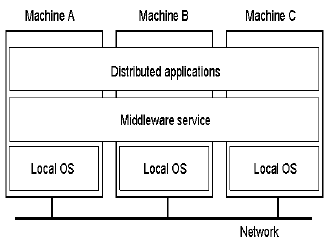
\includegraphics[width=8cm]{img/schemamidd.png}\\
\label{fig:midd}
\caption{Schema di un middleware}
\end{figure}
\subsection{Obiettivi}
La possibilità costruire sistemi distribuiti non implica che tutti i sistemi debbano essere costruiti come sistemi distribuiti. Per far si che sia utile progettare e costruire un sistema distribuito dobbiamo rispettare alcune caratteristiche. un sistema distribuito dovrebbe:
\begin{itemize}
\item rendere le risorse facilmente accessibili,
\item nascondere il fatto che le risorse sono distribuite sulla rete,
\item essere aperto,
\item essere scalabile.
\end{itemize}
\subsubsection{Accessibilità delle risorse}
L'obiettivo principale di un sistema distribuito è quello di rendere facile l'accesso alle risorse remote e condividerle in maniera efficiente e controllata.\\
Ma che cosa intendiamo per "risorse"? Con il termine \emph{risorse} possiamo indicare qualsiasi cosa, alcuni esempi tipici sono stampanti, computer, dati, file, pagine web o intere reti.
Le ragioni che portano a voler condividere le risorse sono molteplici, la prima è sicuramente quella economica, pensiamo ad esempio a ricercatori che condividono un super-computer o ad una stampante condivisa in un ufficio. Inoltre, la connessione di più utenti facilita la collaborazione come avviene nei \textbf{groupware} dove gruppi di persone lavorano insieme anche stando in diverse parti del mondo.\\
Tutto questo incremento di connessione e collaborazione dovrebbe portare però ad una necessaria crescita anche in termini di sicurezza, anche se nella pratica attuale tale incremento nei sistemi di sicurezza non è ancora avvenuto; non è raro trovare sistemi in cui password e altre informazioni sensibili sono inviate come testo in chiaro. Altri problemi legati alla sicurezza sono l'aumento delle \emph{junk mail} o mail di \emph{spam} e l'invio e la raccolta di informazioni riguardanti l'utente per creare un profilo mentre è connesso.
\subsubsection{Trasparenza}
Uno degli obiettivi principali in  un sistema distribuito è quello di nascondere che i processi e le risorse sono distribuiti. Un sistema in grado di presentarsi come un singolo computer è detto \textbf{trasparente}.\\
Possiamo catalogare la trasparenza in diversi tipi in quanto questo concetto può riguardare molti aspetti di un sistema distribuito.\\
La \textbf{trasparenza all'accesso} riguarda le differenze nella rappresentazione dei dati e la modalità di accesso alle risorse da parte degli utenti. Ovvero si desidera nascondere le differenze nelle macchine e trovare un accordo nella rappresentazione dei dati.
Un altro importante tipo di trasparenza è la \textbf{trasparenza di ubicazione} che si prefigge l'obiettivo di nascondere agli utenti la localizzazione di una risorsa. I \emph{nomi} in questa tipo di trasparenza giocano un ruolo importante in quanto è possibile raggiungere tale trasparenza assegnando ad ogni risorsa un nome logico indipendente dalla sua locazione, un esempio di tale tecnica sono gli \emph{URL}.\\
Alcuni sistemi distribuiti che consentono lo spostamento delle risorse senza compromettere la possibilità di accesso devono fornire la \textbf{trasparenza alla migrazione}. Nel caso in cui le risorse possono essere spostate \emph{durante} l'utilizzo senza che utenti o applicazioni notino tale spostamento si deve garantire anche la \textbf{trasparenza al riposizionamento}.\\
La \textbf{trasparenza alla replica} riguarda la possibilità di fornire una o più copie della stessa risorsa per aumentarne la disponibilità e migliorare le prestazioni, tutto questo nascondendo all'utente il fatto che la risorsa è replicata.\\
Come già detto l'obiettivo principale dei sistemi distribuiti è la condivisione di risorse, ma questa porta in alcuni casi ad avere una condivisione di tipo \emph{competitivo} ovvero, più utenti vorrebbero accedere alle stesse risorse (es. una tabella di un database) tutto ciò deve essere evitato tramite la \textbf{trasparenza alla concorrenza} che deve lasciare la risorsa in uno stato consistente. Questa consistenza può essere ottenuta tramite diverse meccanismi tra cui ad esempio il \emph{locking} nel quale gli utenti ottengono a turno l'accesso esclusivo ad una risorsa.\\
Per introdurre l'ultimo tipo di concorrenza partiamo da un'altra definizione di sistema distribuito
\begin{center}
\emph{Ne apprendi l'esistenza quando il crash di un computer di cui non hai mai sentito parlare ti impedisce di portare a termine qualunque lavoro}
\end{center}
Questa definizione pone un altro aspetto importante della progettazione di un sistema distribuito, quello della gestione dei guasti; rendere un sistema \textbf{trasparente ai guasti} significa far si che un utente non si renda conto che una risorsa smette di funzionare correttamente. La difficoltà più grande è distinguere quando una risorsa è morta da quando è semplicemente molto lenta.\\
Sebbene in generale si preferisce avere sistemi trasparenti ci sono situazioni in cui nascondere completamente agli utenti la distribuzione del sistema non è una buona idea. Come nel caso si voglia contattare un servizio che sta dall'altra parte del mondo e si voglia una risposta in un tempo inferiore ai 35ms; o quando si vuole che due repliche siano sempre consistenti, nel caso di server in due continenti diversi un aggiornamento potrebbe richiedere alcuni secondi.\\
Il problema principale che limita però la trasparenza è la trasparenza stessa, infatti, ammettendo che la completa trasparenza di un sistema è \emph{impossibile} è \emph{saggio} cerca di ottenerla a tutti i costi? Rendere la distribuzione esplicita può aiutare gli utenti a capire eventuali comportamenti \emph{anomali} del sistema.
\subsubsection{Apertura}
un altro obiettivo dei sistemi distribuiti è l'apertura. un sistema distribuito \textbf{aperto} è un sistema che offre servizi rispettando delle regole standard che descrivono la sintassi e la semantica dei servizi stessi.\\
Nei sistemi distribuiti i servizi sono descritti tramite \textbf{interfacce} per lo più utilizzando un linguaggio denominato \emph{IDL (interface description language)} che però descrive soltanto la sintassi delle interfacce, ovvero, il nome delle funzioni e i tipi di parametri, i valori di ritorno o le possibili eccezioni sollevate. Per la descrizione di che cosa fa il servizio, invece, si usa solitamente il linguaggio naturale.\\
Se l'interfaccia è ben specificata un processo che ha bisogno di una determinata interfaccia può comunicare con un altro processo che implementa tale interfaccia; inoltre, consente a due processi distinti di implementare tale interfaccia in due modi completamente diversi, il che porta a due sistemi distribuiti che però  operano allo stesso modo.\\
Una specifica però deve essere \emph{completa} e \emph{neutrale}, completa significa che viene specificato tutto ciò che è necessario per realizzare un'implementazione, ma ottenere la completezza è molto difficile e perciò di solito un programmatore deve aggiungere dettagli specifici dell'implementazione. Per neutrale si intende, invece, che la specifica non deve imporre dettagli sull'implementazione. Completezza e neutralità portano ad altre due importanti caratteristiche che i sistemi distribuiti dovrebbero soddisfare, \textbf{interoperabilità} che significa che due implementazioni di vendor diversi possono collaborare e coesistere basandosi unicamente su di uno standard comune. \textbf{Portabilità} indica la possibilità di eseguire un applicazione scritta per un sistema distribuito $A$ su di un sistema distribuito $B$ senza dover apportare modifiche all'applicazione.\\
Infine un altro obiettivo che i sistemi distribuiti dovrebbero prefissarsi è che l'aggiunta o la sostituzione di componenti dovrebbe risultare facile e non influire sui componenti già presenti; questa caratteristica sta ad indicare che il sistema distribuito è \textbf{ampliabile}.
Per ottenere la flessibilità in un sistema aperto è fondamentale che esso sia organizzato come un insieme di componenti piccolo e e facilmente sostituibile e adattabile. Ma questo comporta fornire le interfacce non solo dei componenti che si interfacciano direttamente con gli utenti ma anche dei componenti interni.
\subsubsection{Scalabilità}
La scalabilità sta diventando uno degli aspetti più importanti dei sistemi distribuiti a causa della grande diffusione di internet. Esistono diversi tipi di scalabilità la prima si ha quando un sistema è scalabile rispetto alla sua dimensione il che significa che possiamo aggiungere utenti e risorse. Un sistema può essere scalabile geograficamente quando utenti e risorse sono situati in luoghi molto lontani.
Ed, infine, un sistema può essere scalabile anche dal punto di vista dell'amministrazione ovvero quando comprende molte infrastrutture indipendenti rimane comunque facile da gestire.\\
La scalabilità richiede di affrontare molti problemi. Prendiamo ad esempio la scalabilità rispetto alla dimensione, alcuni servizi in un sistema distribuito possono essere forniti da un unico server questo fa si che aggiungendo utenti quel particolare server diventa un collo di bottiglia per l'intero sistema. A volte l'uso di un solo server è inevitabile come nel caso della gestione di dati sensibili.
Per quanto riguarda la scalabilità a livello geografico anch'essa comporta innumerevoli problemi, infatti, la maggior parte dei sistemi distribuiti che lavorano su LAN si basano sulla comunicazione \textbf{sincrona} nella quale un \emph{client} richiede una risorsa e resta in attesa che tale risorsa sia disponibile. Questo meccanismo non è applicabile per sistemi globali nei quali la comunicazione tra due computer può richiedere anche qualche millisecondo. In oltre si deve tener conto che la comunicazione su WAN(\emph{wide area network}) è inaffidabile e praticamente sempre punto a punto (\emph{point-to-point}). Al contrario le reti locali più affidabili permettono anche il \emph{broadcasting} ovvero l'invio simultaneo a tutte le macchine delle rete dello stesso messaggio.\\
Dopo aver visto i problemi di scalabilità ci chiediamo come risolvere tali problemi nei sistemi distribuiti. I problemi di scaling nei sistemi distribuiti si presentano come problemi nelle prestazioni dovuti alle limitate capacità dei server. Ad oggi esistono soltanto tre tecniche di \emph{scaling}: nascondere le latenze, la distribuzione e la replica.\\
Nascondere le latenze permette di ottenere la scalabilità geografica; l'idea di base è quella di limitare il più possibile i tempi di attesa delle risposte dai servizi remoti. Alcune possibili soluzioni sono anticipare il più possibili la richiesta al server remoto e durante l'attesa della risposta svolgere qualche altra operazione; questo tipo di comunicazione è detta \textbf{comunicazione asincrona}. Quando arriva una risposta l'applicazione si interrompe e viene richiamato un gestore (\emph{handler}) speciale per completare la richiesta sollevata.
Inoltre la comunicazione asincrona è spesso utilizzata nei sistemi \emph{batch} e nelle applicazioni \emph{parallele}.\\
Un'altra soluzione è quella di eseguire un \emph{thread} per la richiesta il quale, anche se si blocca, permette agli altri thread di proseguire.\\
Esiste una classe di applicazioni, però, che non può utilizzare la comunicazione asincrona, questo tipo di applicazioni sono le applicazioni \emph{interattive} nelle quali il client dopo aver effettuato una richiesta ad un server remoto non ha niente di meglio da fare che aspettare la risposta. In questo caso l'unica cosa da fare è limitare il tempo di attesa e per fare ciò solitamente si sposta il carico di lavoro computazionale che solitamente è svolto dal server sul client. Come ad esempio nel caso di compilazione di \emph{form} per un accesso alla base di dati. Si può inviare al server ogni campo della form per poi aspettare dal server la conferma della correttezza dei dati, oppure, più efficiente è far controllare direttamente al client la correttezza dei dati ed inviare al server l'intera form completa.\\
Un'altra soluzione ai problemi di scalabilità è la \textbf{distribuzione} che comporta prendere un componente spezzarlo in parti più piccole e distribuire tali parti nel sistema. Un esempio molto noto di questo tipo di tecnica è il DNS (\emph{domain name system}. Lo spazio dei nomi è organizzato in un albero dei \emph{domini} divisi in zone non sovrapposte. I nomi di ogni zona sono gestiti da un unico server.\\
L'ultima tecnica di scalabilità è la \textbf{replicazione} che consiste nel duplicare quelle risorse che sono maggiormente richieste in modo da evitare colli di bottiglia e bilanciare il carico sulle risorse.
\subsubsection{Tranelli}
I sistemi distribuiti si differenziano dal software tradizionale in quanto sono i componenti sono sparsi per la rete. Il fatto di non tenere conto di questa dispersione in fase progettuale rende i sistemi inutilmente complessi. Questi errori sono dovuti a delle ipotesi (false) che ognuno fa quando progetta un'applicazione distribuita:
\begin{enumerate}
\item La rete è affidabile
\item La rete è sicura
\item La rete è omogenea
\item La topologia non cambia
\item La latenza è zero
\item L'ampiezza di banda è infinita
\item Il costo di trasporto è zero
\item C'è un solo amministratore
\end{enumerate}
\subsection{Tipi di sistemi distribuiti}
Esistono diverse categorie di sistemi distribuiti 
\subsubsection{Sistemi di calcolo distribuiti}
Una classe di sistemi distribuiti è quella utilizzata per calcoli ad alte prestazioni; questa categoria può essere divisa in due sottogruppi. Nei \textbf{sistemi di calcolo a cluster} l'hardware è composto da una serie di workstation connessi ad una rete locale ad alta velocità e in cui ogni nodo ha lo stesso sistema operativo. Nei \textbf{sistemi con tecnologia grid} invece, si intendono sistemi distribuiti costruiti come un gruppo di computer risiedenti in domini di amministrazione diversi con hardware e software differenti.
\paragraph{Sistemi di calcolo a cluster} I sistemi di calcolo a \emph{cluster} divennero popolari quando il rapporto prezzo/prestazioni delle \emph{workstation} divenne vantaggioso. In quasi tutti i casi i sistemi di calcolo a cluster sono utilizzati per per la programmazione parallela.\\
Un esempio di sistema a cluster molto diffuso è il \textbf{Beowolf} un sistema basato su linux in cui l'accesso al sistema avviene tramite un singolo nodo principale, che gestisce l'allocazione dei programmi sui nodi. In realtà il nodo master esegue il \emph{middleware} necessario per l'esecuzione dei programmi e la gestione del cluster. Una parte fondamentale di questo middleware sono le librerie con il quale è sviluppato che forniscono solo funzionalità di comunicazione basate sui messaggi e non sono in grado di gestire errori, sicurezza ecc.\\
Un altro sistema cluster molto diffuso è il \textbf{MOSIX} che fa sembrare il cluster un singolo sistema offrendo così ai programmi la trasparenza di distribuzione.
\paragraph{Grid computing} Al contrario dei sistemi di calcolo a cluster in cui  i componenti hardware sono omogenei nei sistemi \emph{Grid Computing} vi è un alto livello di eterogeneità sia hardware sia software.\\
Solitamente nella tecnologia grid le risorse di diverse aziende vengono unite per consentire la collaborazione che viene anche detta \textbf{organizzazione virtuale}.
\subsubsection{Sistemi informativi basati sulle imprese}
Un'altra classe di sistemi distribuiti si trova in strutture aziendali che si sono confrontate con una gran abbondanza di applicazione in rete ma per le quali l'interoperabilità non è stata facile. In alcuni casi l'integrazione riguardava solamente un server che veniva contattato da diversi client i quali confezionavano una richiesta e la inviavano a tale server. Un'integrazione più approfondita avrebbe permesso ai client di confezionare una richiesta diretta a molteplici server che avrebbero eseguito un \textbf{applicazione distribuita}.
\paragraph{Sistemi transazionali} Sono sistemi incentrati su applicazioni relative a basi di dati. In pratica le operazioni sulle basi di dati sono portate a termine sotto forma di \textbf{transazioni}. In un sistema distribuito transazionale abbiamo la particolarità che all'interno di una transazione possiamo avere delle chiamate a procedura remote ottenendo così un sistema \textbf{RPC transazionale}.
\subsubsection{Sistemi distribuiti pervasivi}
I sistemi distribuiti visti fin qui hanno la particolarità di essere caratterizzati dalla stabilità: i nodi sono fissi ed hanno a disposizione una connessione di alta qualità. Con l'introduzione di dispositivi mobili ed embedded però abbiamo a che fare con sistemi distribuiti in cui la caratteristica principale è l'instabilità; tali sistemi sono detti \textbf{sistemi distribuiti pervasivi}. I sistemi pervasivi hanno delle caratteristiche particolari, intanto non esiste un amministratore umano ma dopo una prima configurazione da parte del proprietario tali sistemi devono adattarsi al meglio all'ambiente circostante. Inoltre tali sistemi devono avere tre requisiti fondamentali:
\begin{itemize}
\item accettare cambi di contesto
\item incoraggiare la composizione \emph{ad-hoc}
\item riconoscere la condivisione di default
\end{itemize}
Ovvero un dispositivo deve essere a conoscenza che il suo ambiente è in costante cambiamento e che i dispositivi che compongono il sistema saranno utilizzati in modo diverso da utenti diversi.
In questo tipo di sistemi non vi è alcun tipo di trasparenza, bensì la distribuzione dei dati dei processi e del controllo è intrinseca nei sistemi ed è quindi più efficiente esporla che nasconderla.
Alcuni esempi di sistemi pervasivi sono:
\begin{itemize}
\item Sistemi domestici
\item Sistemi elettronici per l'assistenza sanitaria
\item Reti di sensori
\end{itemize}